%-------------------------------------------------
%	Version: 0.0
%	fecha de entrega
%
%-------------------------------------------------

\documentclass[11pt]{report}

%packages
\usepackage{graphicx}
\usepackage{subcaption}

\usepackage[utf8]{inputenc}
\usepackage[spanish, es-nodecimaldot]{babel}
\usepackage{setspace}
\usepackage{ragged2e}

\usepackage{amsmath}
\usepackage{amsthm}
\usepackage{amssymb}
\usepackage{mathtools}
\usepackage{siunitx}
\usepackage[thinc]{esdiff} %derivadas faciles
\usepackage{physics} %algunos simbolos de derivadas

%path donde se encuentran las imagenes
\graphicspath{ {./figuras/} }

%---------------------------------------------------------------
%ABREVIACIONES DE COMANDOS

\theoremstyle{plain}
\newtheorem{thm}{Teorema}[chapter] % reset theorem numbering for each chapter

\theoremstyle{definition}
\newtheorem{defn}[thm]{Definición} % definition numbers are dependent on theorem numbers
\newtheorem{exmp}[thm]{Ejemplo} % same for example numbers

\newcommand{\chaptercontent}{
\section{Basics}
\begin{defn}Here is a new definition.\end{defn}
\begin{thm}Here is a new theorem.\end{thm}
\begin{thm}Here is a new theorem.\end{thm}
\begin{exmp}Here is a good example.\end{exmp}
\subsection{Some tips}
\begin{defn}Here is a new definition.\end{defn}
\section{Advanced stuff}
\begin{defn}Here is a new definition.\end{defn}
\subsection{Warnings}
\begin{defn}Here is a new definition.\end{defn}
}

\usepackage{biblatex}
%\addbibresource{Tarea1.bib}

\begin{document}

\begin{titlepage}
\title{Titulo_del_trabajo}

%-------------------------------------------------
%PORTADA
%-------------------------------------------------

	\centering
	{\scshape\LARGE Universidad Autónoma de Yucatán  \\ Facultad de ingeniería\par}
	\vspace{1cm}
	{\scshape\Large Propiedades electrónicas y magnéticas de los materiales\par}
	\vspace{1.5cm}
	{\huge\bfseries Apuntes de clase\par}
	\vspace{0.7cm}
	{\begin{figure}[!h]
	\centering
    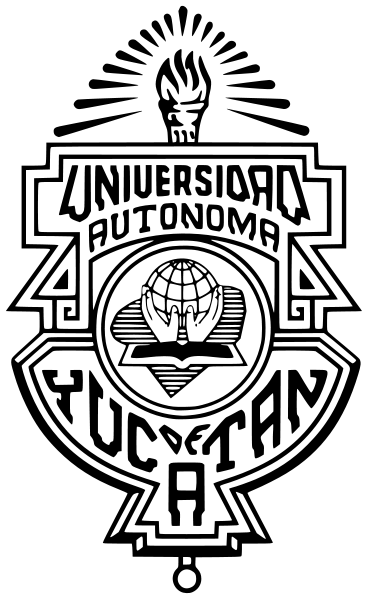
\includegraphics[scale=0.3]{UADY.png}
	\end{figure}}
	\vspace{0.7cm}
	{\Large\itshape Erick Al. Casanova Cortés\par}
	{\Large\itshape Matricula: 15014866\par}
	\vfill
	{\scshape\Large Docente\par
	Dr. Milenis Acosta\par}
	\vfill
	{\Large{\bfseries Fecha de modificación: \today } }

	\vfill
	
\end{titlepage}

%-------------------------------------------------
%Inicio del documento
%-------------------------------------------------

\tableofcontents

%-------------------------------------------------
%Introducción
%-------------------------------------------------

\chapter{Introducción}
La primera clase solo fue presentación y hablamos sobre conceptos que vamos a ver durante el curso

La formativa se encontró en la plataforma, pero dijo que se trabajaran en proyectos y un examen del bloque 1, y otro de la parte magnética
%-------------------------------------------------
%Semiconductores
%-------------------------------------------------
\chapter{Semiconductores}

\section{Tarea preclase}
¿Qué área de interés tienes? Buscar un material semiconductor de esa área, ¿para qué sirve? ¿Qué valor de gap tiene?\\

\textbf{Respuesta}\\

Me interesa ciencia de datos, en sí muchos semiconductores están en el área debido a las herramientas que se utilizan para el análisis y tratamiento. Un ejemplo puede ser silicio, un material bastante utilizado en los procesadores de las computadoras, el uso de un semicondutor en este artefacto es por el hecho de dichos componentes manejan un sistema binario, el cual puede ser interpretado como el paso o el aislamiento de la carga eléctrica. El valor de band gap del silicio es de 1.11eV

%-------------------------------------------------
%Dieléctricos
%-------------------------------------------------
\chapter{Dieléctricos}

%-------------------------------------------------
%Ferroelectricidad y piezoelectricidad
%-------------------------------------------------
\chapter{Ferroelectricidad y piezoelectricidad}

%-------------------------------------------------
%Diamagnetismo y paramagnetismo
%-------------------------------------------------
\chapter{Diamagnetismo y paramagnetismo}


%-------------------------------------------------
%Final del documento
%-------------------------------------------------

\end{document}
